\documentclass{article}

\usepackage[utf8]{inputenc}
\usepackage{graphicx}
\graphicspath{ {Project2/figures/} }
\usepackage{float}
\usepackage{listings}
\usepackage{amsmath}
\usepackage{amssymb}
\usepackage{mathtools}
\usepackage{commath}
\usepackage{tabularx}
\usepackage[ruled,vlined]{algorithm2e}
\usepackage{caption}
\usepackage{subcaption}
\usepackage[outputdir=../]{minted}
\usepackage{verbatim}
\usepackage{tikz}
\usepackage{bm}




\usepackage{amsthm}
\usepackage{enumitem}
\usepackage{breakcites}

\newtheorem{theorem}{Theorem}[section]
\newtheorem{lemma}[theorem]{Lemma}
\theoremstyle{definition}
\newtheorem{definition}{Definition}[subsection]


\bibliographystyle{apalike}
\usepackage{hyperref}
\hypersetup{breaklinks=true,colorlinks=true,linkcolor=blue,citecolor=blue,filecolor=magenta,urlcolor=blue}

\DeclareMathOperator*{\argmax}{arg\,max}
\DeclareMathOperator*{\argmin}{arg\,min}
\DeclareMathOperator*{\sgn}{sgn}
\DeclareMathOperator*{\Bias}{Bias}
\DeclareMathOperator*{\Var}{Var}


\title{Classification and Regression}
\author{Femtehjell, Hoel, Otterlei and Steeneveldt}

\date{October 2023}


\def\@bibdataout@aps{%
\immediate\write\@bibdataout{%
@CONTROL{%
apsrev41Control%
\longbibliography@sw{%
    ,author="08",editor="1",pages="1",title="0",year="1"%
    }{%
    ,author="08",editor="1",pages="1",title="",year="1"%
    }%
  }%
}%
\if@filesw \immediate \write \@auxout {\string \citation {apsrev41Control}}\fi
}

\begin{document}

\setminted[python]{frame=lines,
    framesep=2mm,
    linenos,
    fontsize=\footnotesize,
    mathescape=true,
    escapeinside=||
}

\maketitle
\begin{figure}[H]
    \centering
    
\includegraphics[scale=0.5]{1797261_uio-logo.png}
\end{figure}
\newpage
\tableofcontents
\listoffigures


\newpage

\begin{abstract}
    The abstract will go here
\end{abstract}

\section{Introduction}
In the 1940's, Warren McCullouch and Walter Pitts came up with a mathematical model to describe the neuron cell in the brain. They called this model threshold logic \textbf{(legg til kilde)}. Later, this model became the perceptron model \textbf{(dobbelsjekk} fakta) and when added more layers, became the multi-layer perceptron model, the first model of a feed forward neural network (FFNN). \\
... \\
In scientific research, the use of neural networks has exploded and the set of variations on different architectures keeps expanding. FFNN is the biggest category of artificial neural network (ANN) and other types of ANNs, such as recurrent neural networks, even builds upon it. This naturally makes it interesting to see how one can build a good FFNN model. \\
This project will first take a look at the theory behind neural network. Starting with a theoretical aspect of optimization and moving to the theoretical models of feed forward neural network and logistic regression. Then moving on to the methods used in the project to test different techniques, as well as the results from these techniques. Further, the results will be discussed and lastly a conclusion of the project will be (something, cant find the word).

\newpage

\section{Theory}
\subsection{Regression}

\subsubsection{OLS}
Ordinary least squares is a method used to best fit a line to a set of data points. It minimizes the sum of squared residuals, which means it finds the distance between the input data points and the points along the line. The goal is to find the best relationship between a independent variable $\mathbf{x}$ (the input data) and a dependent variable $\mathbf{y}$ (the correct data).
Let $f: X \rightarrow Y$ be a continuous function such that
\begin{equation*}
    \mathbf{y} = f(\mathbf{x}) + \epsilon
\end{equation*}
where $\mathbf{y} \in Y$ is our correct data, $\mathbf{x} \in X$ is the input data and $\epsilon$ is the error term given as $\epsilon \sim N(0,\sigma^2)$. Looking to approximate $f$, we consider $n$ samples and assume that there are $p$ characteristics which define each of the samples, such that $y_i = f(\mathbf{x}_i) + \epsilon_i$, with $\mathbf{x}_i = [x_{i,0},x_{i,1},...,x_{i,p-1}]$. The approximation of $f$ should give us $\mathbf{\Tilde{y}}$ such that $\tfrac{1}{n}(\mathbf{y} - \mathbf{\Tilde{y}})$ is minimized. \\
... \\
We assume a linear relationship such that $y_i = \mathbf{x}_i \cdot \bm{\beta} + \epsilon$. We can write this more compact as
\begin{equation*}
    \mathbf{y} =
    \begin{bmatrix}
        x_{0,0} & x_{0,1} & \ldots & x_{0, p-1} \\
        x_{1,0} & x_{1,1} & \ldots & x_{1, p-1} \\
        \vdots & \vdots & \ddots & \vdots \\
        x_{n,0} & x_{n,1} & \ldots & x_{n, p-1}
    \end{bmatrix}
    \begin{bmatrix}
        \beta_0 \\
        \beta_1 \\
        \vdots \\
        \beta_{p-1}
    \end{bmatrix}
    +
    \begin{bmatrix}
        \epsilon_0 \\
        \epsilon_1 \\
        \vdots \\
        \epsilon_{p-1}
    \end{bmatrix}
    = \mathbf{X}\bm{\beta} + \epsilon
\end{equation*}
where the $\mathbf{X}$ is called the design matrix and $\bm{\beta}$ is called weights. Wanting to find
\begin{equation*}
    \bm{\hat{\beta}} = \argmin_{\beta \in \mathbb{R}^p}\tfrac{1}{n}(\mathbf{y} - \mathbf{X}\bm{\beta})^T(\mathbf{y} - \mathbf{X}\bm{\beta})
\end{equation*}
and knowing that
\begin{equation*}
    (\mathbf{y} - \mathbf{X}\bm{\beta})^T(\mathbf{y} - \mathbf{X}\bm{\beta}) = \mathbf{y}^T\mathbf{y} - 2\bm{\beta}^T\mathbf{X}^T\mathbf{y} + \bm{\beta}^T\mathbf{X}^T\mathbf{X}\bm{\beta}
\end{equation*}
we can compute the partial derivatives of the above expression and neglect the scaling factor $\tfrac{1}{n}$. This gives us
\begin{gather*}
    \frac{\partial}{\partial \boldsymbol{\beta}} \left( \boldsymbol{y}^T \boldsymbol{y} - 2 \boldsymbol{\beta}^T \textbf{X}^T \boldsymbol{y} + \boldsymbol{\beta}^T \textbf{X}^T \textbf{X} \boldsymbol{\beta} \right) = 0 \\
    -2 \textbf{X}^T \boldsymbol{y} + 2 \textbf{X}^T \boldsymbol{X \beta} = 0 \\
    2 \textbf{X}^T \boldsymbol{X \beta} = 2 \textbf{X}^T \boldsymbol{y} \\
    \boldsymbol{\beta} = \left( \textbf{X}^T \textbf{X} \right)^{-1} \textbf{X}^T \boldsymbol{y}
\end{gather*}
Now we have an analytical expression for the weights, which is what we wanted.
For a more detailed and longer explanation of OLS, including the expectation and variance of OLS, see (project 1 link goes here)

\subsubsection{Ridge}
Overfitting is the concept where the model learns the training data too well, and failing to generalize to other data sets. As an analogy, this would be similar to someone learning what numbered answer to answer on a test instead of actually learning the topic of the test. This can be a challenge in OLS and thus we introduce a regularization term in ridge regression. The new expression to minimize becomes
\begin{equation*}
    \bm{\hat{\beta}} = \argmin_{\beta \in \mathbb{R}^p}\tfrac{1}{n}(\mathbf{y} - \mathbf{X}\bm{\beta})^T(\mathbf{y} - \mathbf{X}\bm{\beta}) + \lambda\bm{\beta}^2
\end{equation*}
where the right hand side multiplies to
\begin{equation*}
    \frac{1}{n}(\mathbf{y}^T\mathbf{y} - 2\bm{\beta}^T\mathbf{X}^T\mathbf{y} + \bm{\beta}^T\mathbf{X}^T\mathbf{X}\bm{\beta}) + \lambda\bm{\beta}^T\bm{\beta}
\end{equation*}
Finding again the partial derivatives, we get
\begin{gather*}
    \frac{\partial}{\partial \boldsymbol{\beta}} \left( \left( \boldsymbol{y} - \textbf{X} \boldsymbol{\beta} \right)^2 + \lambda \boldsymbol{\beta}^2 \right) = 0 \\
    -2 \textbf{X}^T \boldsymbol{y} + 2 \textbf{X}^T \boldsymbol{X \beta} + 2\lambda \boldsymbol{\beta} = 0 \\
    \textbf{X}^T \boldsymbol{X \beta} + \lambda \boldsymbol{\beta} = \textbf{X}^T \boldsymbol{y} \\
    \left(\textbf{X}^T \textbf{X} + \boldsymbol{I}_p \lambda \right) \boldsymbol{\beta} = \textbf{X}^T \boldsymbol{y} \\
    \boldsymbol{\beta} = \left(\textbf{X}^T \textbf{X} + \boldsymbol{I}_p \lambda \right)^{-1} \textbf{X}^T \boldsymbol{y}
\end{gather*}
For a more detailed explanation of ridge regression, see (Project 1 link)

\subsubsection{Logistic regression}
Temporary notes
\begin{itemize}
    \item transformation of a linear model to guarantee that the output is a probability
    \item $p(X) = \frac{e^{b_0 + b_1X}}{1 + e^{b_0 + b_1X}}$
    \item $log(\frac{p(X)}{1 - p(X)})$ (log odds / logit)
    \item using maximum likelihood to estimate parameters
    \item $l(b_0,b_1) = \prod_{i=1}^{n}p(x_i)\prod_{i=1}^{n}(1 - p(x_i))$
    \item joint probability of the observed zeros and ones
\end{itemize} 

\subsection{Optimization}

%%At the core of most issues within machine learning and data analysis, we find an optimization problem.  In a perfect scenario we would like to like to find this analytically, however for various reasons, whether they be computational or purely mathematical in nature, this is often not possible. 
At the core of most issues within machine learning and data analysis, we find an optimization problem. That is we wish to find the minimum of a function. In a perfect scenario we would like to find this analytically, however for various reasons, whether they be computational or purely mathematical in nature, this is often not possible. Therefore we opt for iterative methods instead.
\subsubsection{Gradient descent}

Let  $$f: \mathbf{X}^n \rightarrow \mathbf{Y}$$ be the function we wish to minimize, where $ \mathbf{X} \subseteq \mathbb{R}^n, \mathbf{Y}\subseteq \mathbb{R}$. If $f$ is differentiable the extrema, $f(\mathbf{x^*})$, satisfy $\nabla \mathbf{f(w^*)} = \mathbf{0}$. Let $f(\mathbf{\xi})$ denote a local minima. Then we approximate $\mathbf{\xi}$ by the iteration

\begin{align*} \label{eq:1}
\mathbf{w}_{k+1} =& \mathbf{w}_k - \eta_k \nabla  \mathbf{f(\mathbf{w}_k)}\\
 =& \mathbf{w}_k - \eta_k  \mathbf{g_k}
\end{align*}
The scalar in front of the gradient term, here $\eta_k$, is called the learning rate. If we let it be constant we get gradient descent. For each iteration we move our approximation of the minima in the opposite direction of the gradient; the direction of maximum growth. 

This is also known as simultaneous relaxation and under certain conditions on the Hessian it can be shown that 
$\mathbf{w_k}$ converges to $\mathbf{\xi}$  given that $\mathbf{w_0}$ is close enough to $\xi$ \cite[p.~117--118]{introNumeric}
For non differentiable functions we may still obtain convergence by clever choice of $\eta_k$ and numerical approximations of the gradient. 
\autoref{fig:simple_gradient_descent} shows a simple example of 100 iterations performed on $f(w) = w^2$ with $\eta = 0.01$

\begin{figure}[H]
    \centering
    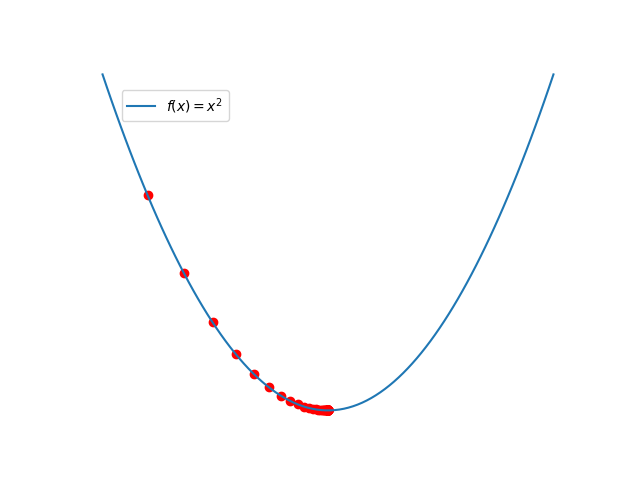
\includegraphics[width=0.68\textwidth]{Project2/figures/simple_gradient_descent.png}
    \caption{Gradient Descent on the function $f(x)=x^2$, starting from $w_0 = -4$ with $\eta = 0.01$, ran for 30 iterations.}
    \label{fig:simple_gradient_descent}
\end{figure}
For this simple example the iteration converged quickly, reaching a absolute value less than 0.001 after only 27 iterations. Gradient descent is not always this efficient. 

The two natural weaknesses of gradient descent are neatly explained in \cite[p.~65--71]{MLRefined}. The first stems from the gradient being always perpendicular to the contour line. This is easily proved through parameterization.


\begin{lemma}
    Let $w(t)$ be a parametrization of a countour surface for a differentiable function $f: X^n \rightarrow Y$. Then $\nabla f \perp w(t) $ 
\end{lemma}

\begin{proof}
$$f(w(t)) = C \Rightarrow \frac{d}{dt} f(w(t)) = 0 \Rightarrow \nabla f(w(t)) \cdot \frac{\partial w(t)}{\partial t} = 0$$
The result follows from $\frac{\partial w(t)}{\partial t}$ being parallel to the contour
\end{proof}

This may lead to Zig-zagging behavior for ill conditioned problems.

\begin{figure}[H]
    \centering
    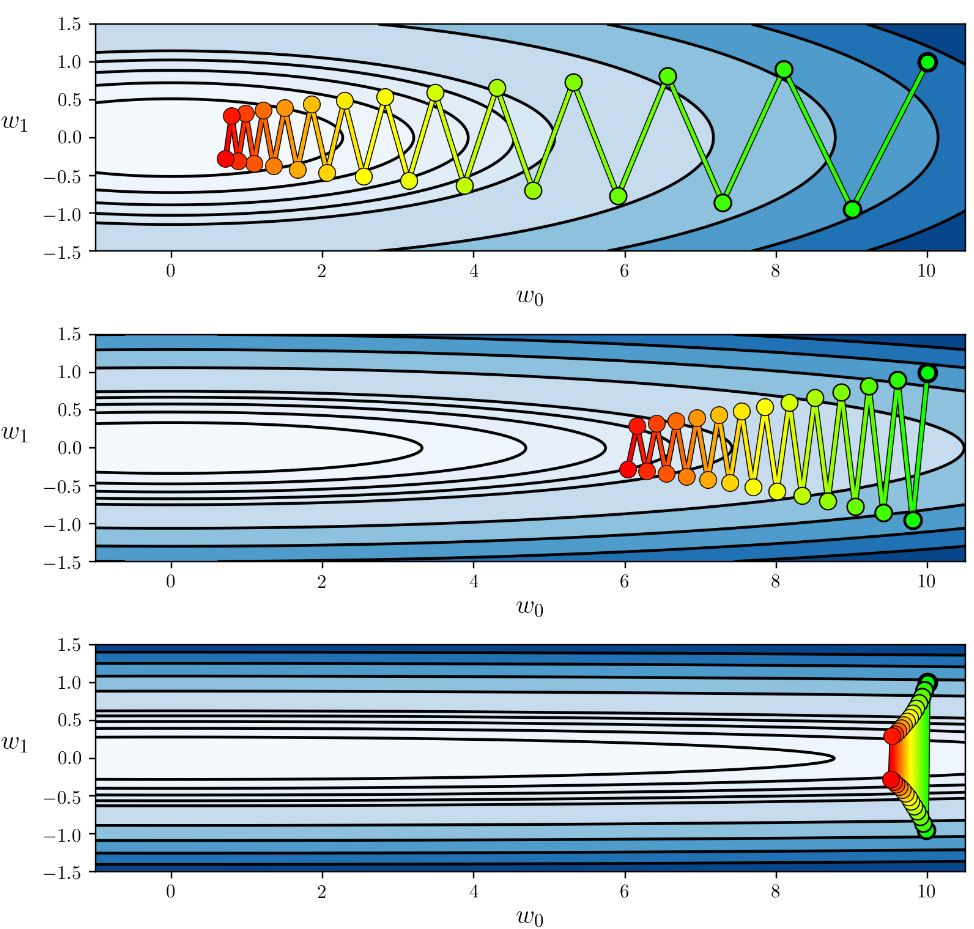
\includegraphics[width=0.9\textwidth]{Project2/figures/Gradient_descent_zigzag.jpeg}
    \caption{Figure 3.13 \cite[p.~68]{MLRefined} illustrating the zig-zagging behavior
of gradient descent.}
    \label{fig:zigzagGradientDescent}
\end{figure}

The other challenge of gradient descent is its slow crawling behaviour in flatter regions of a function such as saddle points.  
This is nicely illustrated by 50 iterations with $\eta = 0.1$ on the function 
\[g(w) =  max^2(0, 1 + (3w - 2.3)^3) + max^2(0, 1 + (-3w + 0.7)^3)\]

\begin{figure}[H]
    \centering
    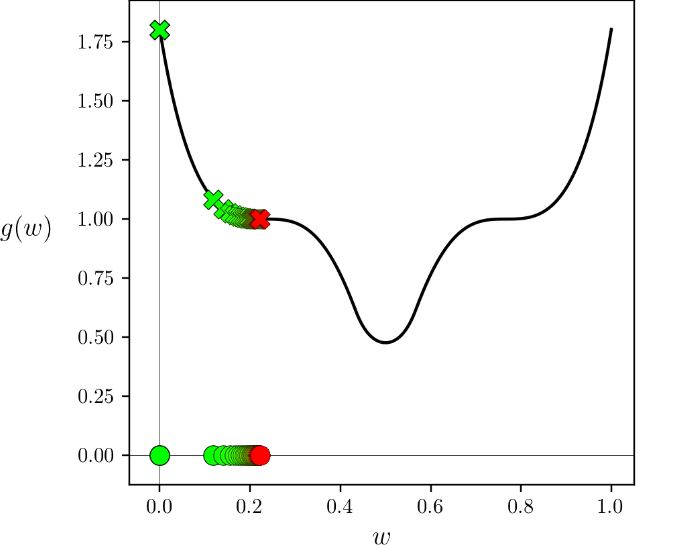
\includegraphics[width=0.7\textwidth]{Project2/figures/Gradient_descent_saddle_crawl.jpeg}
    \caption{Figure 3.14 \cite[p.~70]{MLRefined} illustrating the slow crawling behaviour
of gradient descent.}
    \label{fig:CrawlGradientDescent}
\end{figure}

\subsubsection{Stochastic gradient descent}
Stochastic gradient descent (or SGD) introduces the concept of batching. Instead of computing the gradient for all data points, as is done in deterministic gradient descent, we split the data set into batches (or mini-batches). \\
Let $M$ be the size of the batches and $n$ the number of data points, then the number of batches will be $m = \frac{M}{n}$. In the special case of $M = n$, there is only one batch and SGD becomes "vanilla" gradient descent again. In SGD, the algorithm have an inner loop that iterates $m$ times. For each time a new batch is drawn randomly from the data points and calculates the gradient and updates the learning rate. \\
Let $\mathbf{x_i}$ be the $i_{th}$ batch and $i=1,...,m$, then we can rewrite eq. \autoref{eq:1} as
\begin{align*}
        \mathbf{w_{j+1}} = \mathbf{w_j} - \eta_k\nabla\mathbf{f(x_i)}
\end{align*}
where $j=1,...,m+epochs$. As stated above, the gradient descent finds the local minima $f(\xi)$ by exploitation. This is beneficial for convex functions or if the local minima is already known to be the global minima. For non-convex functions or in the case where the global minima is not known (which is the case most of the time), SGD introduces more exploration. This means that instead of getting stuck in a local minima, by randomness, there is a higher probability of finding the global minima. SGD also have an added bonus that it is dependent on the batch size rather than the data set size. Thus the learning rate can still converge, even if the data set gets large.

\subsubsection{Momentum based gradient descent}
Momentum is an added parameter meant to address these issues of vanilla gradient descent. The iteration is defined as

\begin{align*}
    \mathbf{w_{k+1}} &= \mathbf{w_k} + \mathbf{v_{t+1}}, \\
    \mathbf{v_{t+1}} &= \rho \mathbf{v_t} - \eta \mathbf{g_k}, \hspace{3mm} \mathbf{v_0} = 0
\end{align*}

$\mathbf{v}$ is called the velocity term and $\rho$ is the momentum parameter. $\rho$ can be thought of as the velocities resistance to change while the learning rate ($\eta$) characterizes the influence of the gradient. An intuitive analogy is to think of our descent algorithm as a particle moving on the surface we wish to minimize. The gradient is the force acting on our particle ($\eta$ is its amplifier) and $\rho$ is the mass of the particle. This way our particle might be able to roll past the saddle point in \autoref{fig:CrawlGradientDescent} and obtain a less "zig-zaggy" path in \autoref{fig:ZigZagMomentumGradientDescent}.

\newpage

Here we see momentum gradient descent performed on the same ill conditioned problem as the first panel of \autoref{fig:ZigZagMomentumGradientDescent} with $\rho$ equal to $0, 0.2, 0.7$ respectively

\begin{figure}[H]
    \centering
    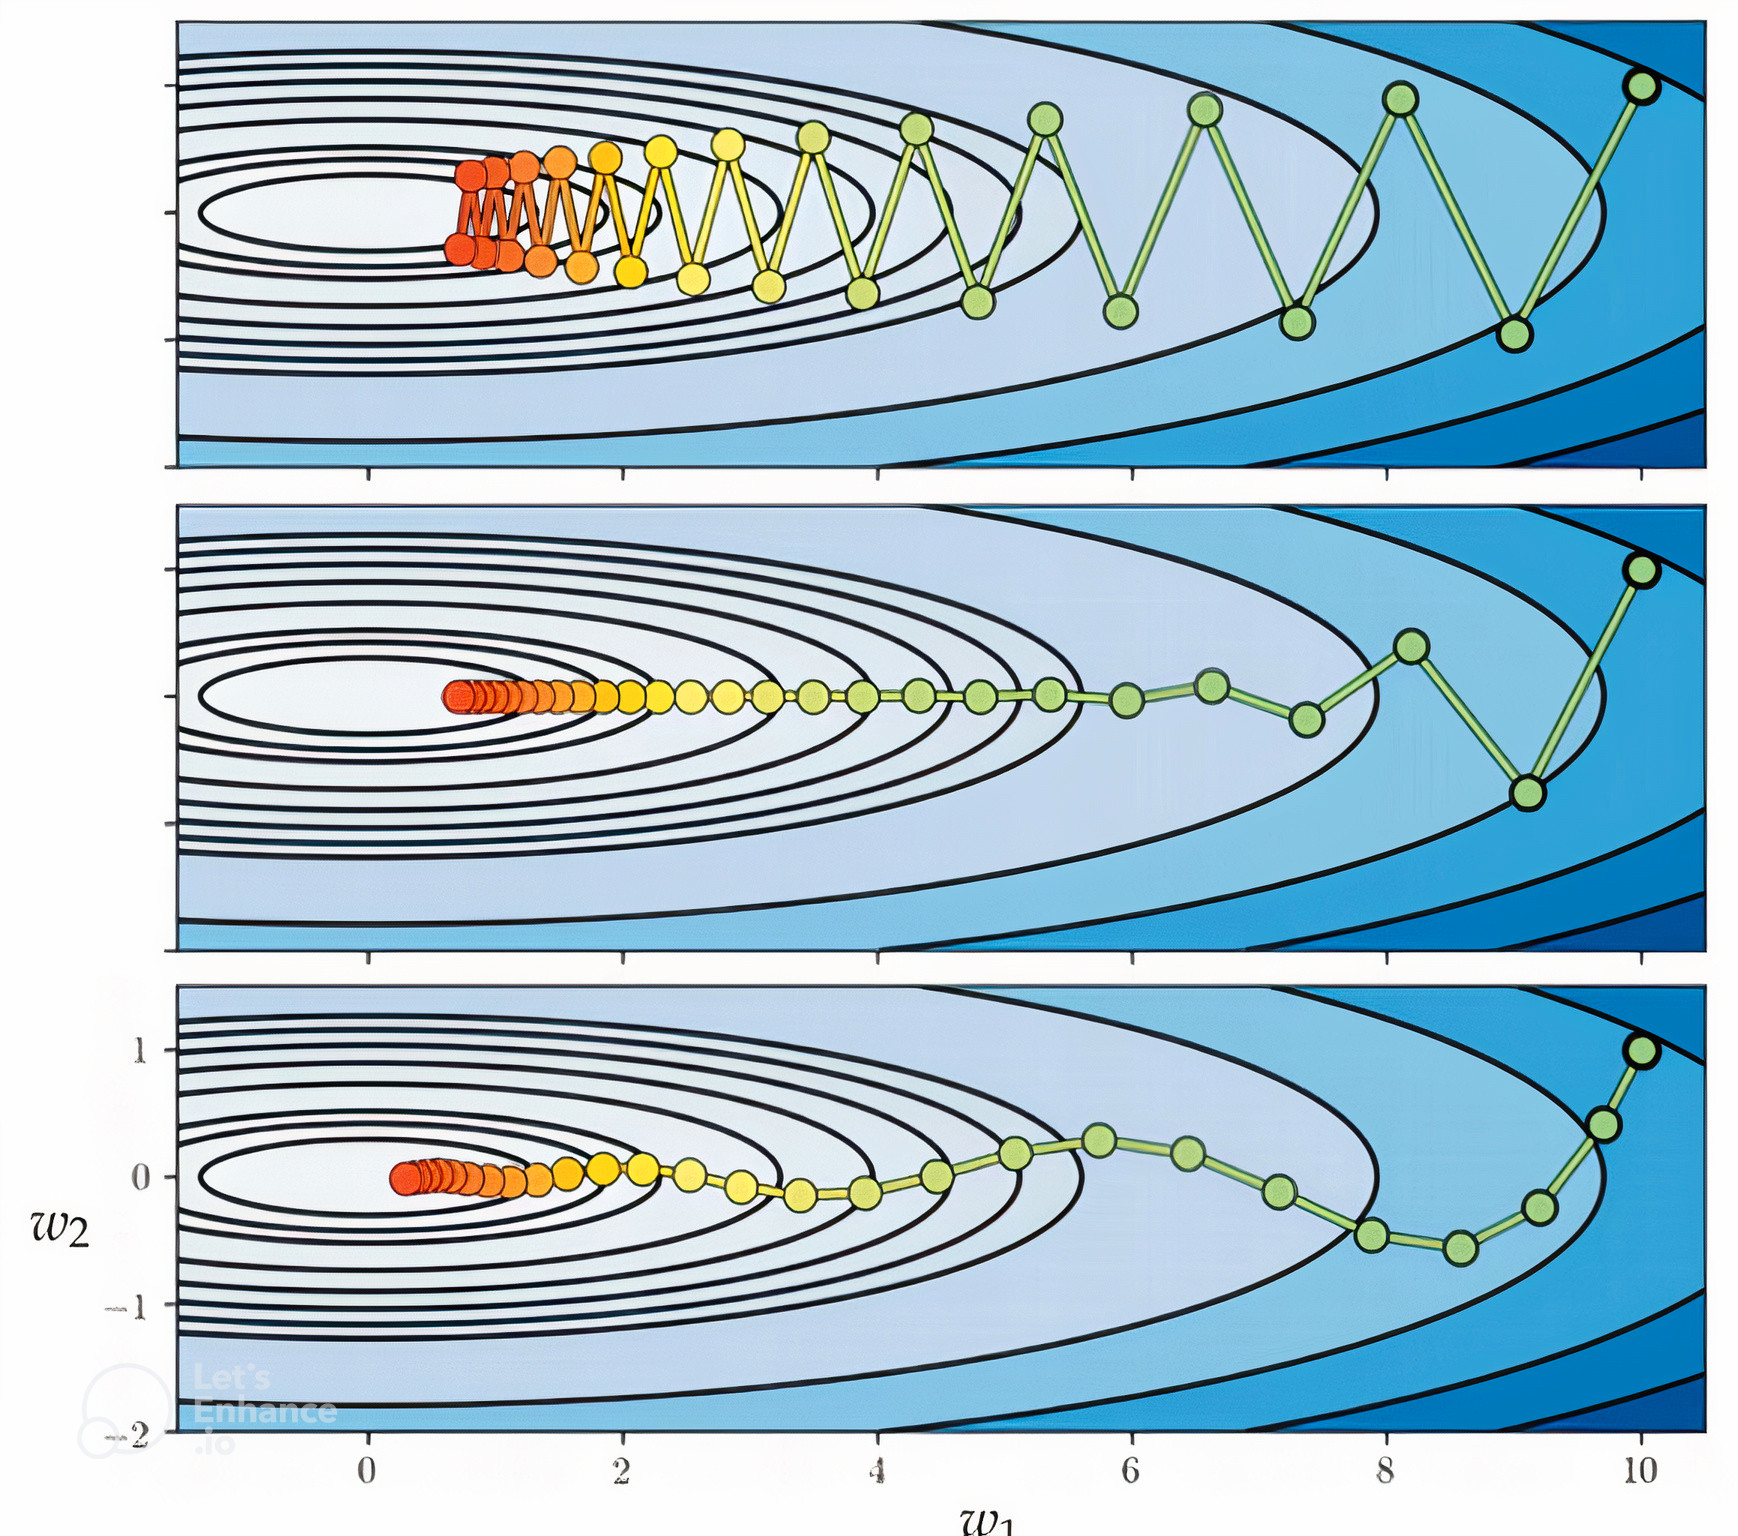
\includegraphics[width=0.8\textwidth]{Project2/figures/momentum_based_gradient_descent_less_zig.jpg.jpg}
    \caption{Figure A3 \cite[p.~478]{MLRefined} The zig-zagging behavior of gradient
descent can be ameliorated using the momentum-accelerated gradient descent}
    \label{fig:ZigZagMomentumGradientDescent}
\end{figure}


\subsubsection{AdaGrad}
The Adaptive gradient optimizer, or AdaGrad was introduced by \cite{duchi2011adaptive} and its update rule is given by

\[ w_{k+1}= w_{k}-\eta \mathbf{G_{k}}^{\circ -1/2} \odot \mathbf{\nabla f(w_k)} \]
where $\odot$ is the Hadamard product, $\circ$ is the Hadamard power. $G_k$ is then the sum of the Hadamard squares of the previous gradients 
\begin{equation}
    G_k = \sum_{i = 0}^k \mathbf{g_i}^{\circ 2} = \sum_{i = 0}^k \mathbf{\nabla f(w_i)}^{\circ 2} = \sum_{i = 0}^k \mathbf{\nabla f(w_i)} \odot \mathbf{\nabla f(w_i)}
\end{equation}

 Element wise we have that $G_{k}^{(n)}$ ( the $n$-th component of $G_k$) is the sum of the squares of the previous gradients in direction $n$
 \[
 G_{k}^{(n)} = \sum_{i=0}^k  \left(g_k^{(n)}\right)^2 
 \]

 Normally a small numerical stabiliser is added to $G_k$ to avoid division by zero
 \[
 w_{k+1}^{(n)}= w_{k}^{(n)}- \frac{\eta}{\delta + \sqrt{G_{k}^{(n)}}} \odot g_k^{(n)}
 \]
 

As $G_k^{(n)}$ increases, the step size in direction $n$ decreases, which reduces the emphasis on that particular direction as it is traversed. This is the core concept of AdaGrad's design. AdaGrad is most effective when two conditions are met: first, when we need to move the same distance in each dimension, and second, when we have an appropriate choice of $\eta$. Opting for a too small $\eta$ could result in the algorithm converging very slowly or coming to a halt due to the decaying step size. Conversely, selecting a too large $\eta$ could lead to also sluggish convergence. Thus, selecting an appropriate value of $\eta$ is vital to ensuring efficient functioning of the algorithm. 


\subsubsection{RMSprop}
RMSprop, root mean square propagation, was first introduced in 2012, in lecture 6 of the Coursera course ``Neural Networks for Machine Learning" by Geoff Hinton
\cite{NNforML-Lecture6} It's update rule is defined as 

\begin{align*}
    \mathbf{v_{k+1}} =& \beta \mathbf{v_{k}} + (1-\beta) \mathbf{g_k}^{\circ 2}\\
    w_{k+1}^{(n)} =& w_k^{(n)} - \frac{\eta}{\delta +  \sqrt{v_{k+1}^{(n)}}} g_k^{(n)}
\end{align*}

 We have chosen to only give the element wise update rule, as for RMSprop, as the vector notation for the final equation is not very pretty. $\delta$ is a numerical stabilizer, $0\leq \beta \leq 1$ and $\mathbf{v_0}$ is usually initialised to the zero vector.
\par
\vspace{1mm}
Like AdaGrad the update keeps some sort of memory of previous gradients. Where $\beta$ can be thought of as the strength of the memory; how much of the previous iterations should impact the next. This allows for some of the same benefits as AdaGrads decaying learningrate.

\subsubsection{ADAM}
Adaprive moment estimation, most commonly known as ADAM. Is a optimization algorithm which combines the some of the aspects from RMSprop with momentum. It's update is given by
\begin{align*}
    \mathbf{m_{k+1}} =& \frac{\beta_1 \mathbf{m_k} + (1- \beta_1) \mathbf{g_k}}{\left(1 - \beta_1^{k+1}\right)}\\
    \mathbf{v_{k+1}} =& \frac{\beta_2 \mathbf{v_k} + (1-\beta_2) \mathbf{g_k}^{\circ 2}}{\left(1-\beta_2^{k+1}\right)}\\
    w_{k+1}^{(n)} =& w_k^{(n)} - \frac{\eta}{\delta + \sqrt{v_{k+1}^{(n)}}} m_{k+1}^{n}
\end{align*}

Here $0 \leq \beta_1,\beta_2 < 1$ 
\par
\vspace{1mm}
Notice that the denominator of $\mathbf{m_{k+1}}$ and $\mathbf{v_{k+1}}$ starts somewhere in $(0,1]$ and then increases to 1 as $k \to \infty$. This gives an amplification of the vectors, which subsides for larger $k$. This is meant to alleviate a bias towards zero as  $\mathbf{m_0}, \mathbf{v_0} = 0$ \cite{kingma2014adam}[section 3]

\subsection{Neural Networks}
% Neural networks are computational systems inspired by the networks of neurons in the brain.

% A neural network mainly consists of an input layer of nodes, a set of weights, an activation function, a hidden layer of nodes and a layer of output nodes. The input nodes are usually called features. Each node is connected to all nodes in the next layer and the edge between them have a weight on it. In the next layer, each input to the node is multiplied with its own weight and then summed together. These nodes are usually what we would call an artificial neuron.\\
% Let $f: X \rightarrow X$ be a function (?), then we can define the artificial neuron as
% \begin{equation*}
%     y = f\left( \sum_{i=1}^{n}w_ix_i \right)
% \end{equation*}
% \\
% $\ldots$\\
Neural networks are computational systems inspired by the networks of neurons within the brain. In the brain, when a neuron receives an electrical impulse above a certain threshold, it sends an electrical signal to the neurons connected to it, causing a chain reaction. In order to mimic this, an artificial neural network is set up with a number of layers, each with a set of artificial neurons. The first layer is commonly called the input layer, which is followed by a number of hidden layers, culminating in the final layer called the output layer.

\begin{figure}[ht]
\centering
\def\layersep{2.5cm}
\def\nodeinlayersep{1.2cm}
\begin{tikzpicture}[shorten >=1pt,->,draw=black!50, node distance=\layersep]
    \tikzstyle{every pin edge}=[<-,shorten <=1pt]
    \tikzstyle{neuron}=[circle, fill=black!25,minimum size=20pt,inner sep=0pt]
    \tikzstyle{input neuron}=[neuron, fill=red!50];
    \tikzstyle{output neuron}=[neuron, fill=orange!50];
    \tikzstyle{hidden neuron}=[neuron, fill=blue!50, minimum size=20pt];
    \tikzstyle{hidden neuron2}=[neuron, fill=blue!50, minimum size=20pt];

    \foreach \name / \y in {0,...,2}
        \node[input neuron] (I-\name) at (0,-\y) {};

    \foreach \name / \y in {0,...,3}
        \path[yshift=0.5cm]
            node[hidden neuron] (H1-\name) at (\layersep,-\y cm) {};

    \foreach \name / \y in {0,...,3}
        \path[yshift=0.5cm]
            node[hidden neuron2] (H2-\name) at (2*\layersep,-\y cm) {};    

    \foreach \name / \y in {0,...,1}
        % \node[output neuron,pin={[pun edge={->}]right:Output \#\y}, right of=H2-2] (O-\name) at (3*\layersep, -\y cm) {};
        \path[yshift=-0.5cm]
            node[output neuron] (O-\name) at (3*\layersep, -\y cm) {};


    \foreach \source in {0,...,2}
        \foreach \dest in {0,...,3}
            \path (I-\source) edge (H1-\dest);

    \foreach \source in {0,...,3}
        \foreach \dest in {0,...,3}
            \path (H1-\source) edge (H2-\dest);

    \foreach \source in {0,...,3}
        \foreach \dest in {0,...,1}
            \path (H2-\source) edge (O-\dest);
\end{tikzpicture}
\caption{Illustration of a fully connected feed-forward neural network with an input layer (red), two hidden layers (blue) and an output layer (orange).}
\label{fig:SimpleFFNN}
\end{figure}

The \textit{feed-forward} neural network (FFNN), was the first, and perhaps simplest, artificial neural network (\textbf{SOURCE}). Each node is connected to nodes in the next layer, with a weight $w \in \mathbb{R}$ attached to each edge. Additionally, we attach one weight $b \in \mathbb{R}$ to the node itself, called the bias. Henceforth, we describe the \textit{fully connected} feed-forward neural network, where the nodes are connected to \textit{all} nodes in the next layer, illustrated in \autoref{fig:SimpleFFNN}.

Information in this network moves from left to right. The value of a node is dependent on the weights and values of the previous layer, as well as the bias. Let $N_l \in \mathbb{N}$ be the number of nodes in layer $l$ with the input layer being $l = 0$. We then calculate
\begin{equation*}
    z_{i}^1 = \sum_{j = 0}^{N_0 - 1} w_{ij}^1 x_j + b_i^1 \qquad \textnormal{for} \ i = 0, 1, \ldots, N_1 - 1,
\end{equation*}
with $w^l_{ij}, b^l_i \in \mathbb{R}$ being the weight connecting nodes $i$ and $j$ in layer $l$ and bias of node $i$, and $x_j \in \mathbb{R}$ being $j$-th input. We call $z$ the activation value. Let $f^l: \mathbb{R} \to \mathbb{R}$ be a function, called the activation function for the $l$-th layer. We calculate the output of the node by $a_i^l = f^l(z_i^l)$. For the following layers, we calculate a \textit{feed-forward pass}
\begin{equation*}
    a_i^l = f^l(z_{i}^l) = f^l \left( \sum_{j = 0}^{N_l - 1} w_{ij}^l a_j^{l-1} + b_i^{l} \right) \qquad \textnormal{for} \ i = 0, 1, \ldots, N_l - 1,
\end{equation*}
illustrated in \autoref{fig:FeedForward}.

\begin{figure}[ht]
\centering
\def\layersep{3cm}
\def\nodeinlayersep{2cm}
\begin{tikzpicture}[shorten >=1pt,->,draw=black!50, node distance=\layersep]
    \tikzstyle{every pin edge}=[<-,shorten <=1pt]
    \tikzstyle{neuron}=[circle, fill=black!25,minimum size=25pt,inner sep=0pt]
    \tikzstyle{input neuron}=[neuron, fill=red!50];
    \tikzstyle{output neuron}=[neuron, fill=orange!50];
    \tikzstyle{hidden neuron}=[neuron, fill=blue!50];

    % Input nodes
    \foreach \name / \y in {0,...,1}
        \node[input neuron] (I-\name) at (0,-\y * \nodeinlayersep) {$x_\y$};

    % Hidden layer
    \foreach \name / \y in {0,...,1}
        \node[hidden neuron] (H-\name) at (\layersep,-\y * \nodeinlayersep) {$a_\y^1$};

    % Output node
    \path[yshift=-0.5 * \nodeinlayersep]
        node[output neuron] (O-0) at (2*\layersep, 0 cm) {$a_0^2$};

    \path[->] 
        % Weights from first input
        (I-0) edge [->] node [midway, above] {$w^1_{0, 0}$} (H-0)
        (I-0) edge [->] node [midway, above] {$w^1_{0, 1}$} (H-1)
        % Weights from second input
        (I-1) edge [->] node [midway, below] {$w^1_{1, 0}$} (H-0)
        (I-1) edge [->] node [midway, below] {$w^1_{1, 1}$} (H-1)
        % Weights to output
        (H-0) edge [->] node [midway, above] {$w^2_{0, 0}$} (O-0)
        (H-1) edge [->] node [midway, below] {$w^2_{1, 0}$} (O-0);

    
    \foreach \source in {0,...,1}
        \foreach \dest in {0}
            \path (H-\source) edge (O-\dest);

    \path[->]
        (H-0) edge [loop above] node [above] {$f\left(z_0^1\right)$} ()
        (H-1) edge [loop below] node [below] {$f\left(z_1^1\right)$} ()
        (O-0) edge [loop above] node [above] {$f\left(z_0^2\right)$} ();

    \node (BH-0) at (0.5*\layersep,  0.5*\nodeinlayersep) {$b_0^1$};
    \node (BH-1) at (0.5*\layersep, -1.5*\nodeinlayersep) {$b_1^1$};
    \node (BO-0) at (1.5*\layersep, -0.5*\nodeinlayersep) {$b_0^2$};

    \path[->]
        (BH-0) edge (H-0)
        (BH-1) edge (H-1)
        (BO-0) edge (O-0);
\end{tikzpicture}
\caption{Illustration of a feed-forward pass in a neural network with two inputs (red), two hidden nodes (blue), and one output node (orange).}
\label{fig:FeedForward}
\end{figure}

We gather the weights connecting the $l$-th and $(l-1)$-th layers in a $N_{l} \times N_{l-1}$ matrix $\mathbf{W}_l$, and the biases and outputs in $N_l \times 1$ column vectors $\mathbf{b}_l, \mathbf{y}_l$ as follows.
\begin{equation*}
    \mathbf{W}_l = 
    \begin{bmatrix}
        w_{0,0} & w_{0,1} & \ldots & w_{0,N_{l-1}} \\
        w_{1,0} & w_{1,1} & \ldots & w_{1,N_{l-1}} \\
        \vdots & \vdots & \ddots & \vdots \\
        w_{N_{l},0} & w_{N_{l},1} & \ldots & w_{N_{l},N_{l-1}} \\
    \end{bmatrix}
    \qquad
    \mathbf{b}_l =
    \begin{bmatrix}
        b_0^l \\ b_1^l \\ \vdots \\ b_{N_l}^l
    \end{bmatrix}
    \qquad
    \mathbf{y}_l =
    \begin{bmatrix}
        y_0^l \\ y_1^l \\ \vdots \\ y_{N_l}^l
    \end{bmatrix}
\end{equation*}
We can then simplify the summation to get $\mathbf{z}_l = \mathbf{W}_l \mathbf{y}_{l-1} + \mathbf{b}_l$. We then extend the function $f^l: \mathbb{R} \to \mathbb{R}$ to the function $F^l: \mathbb{R}^{N_l \times 1} \to \mathbb{R}^{N_l \times 1}$ by defining
\begin{equation*}
    F^l(\boldsymbol{x}) = \left[ f^l \left( x_0 \right), \ f^l \left( x_1 \right), \ \ldots, \ f^l \left( x_{N_l - 1} \right) \right]^T,
\end{equation*}
such that the function operates elementwise. For simplicity sake, this function $F^l$ will also be notated $f^l$.

We define the realization of our neural network as the function $\mathcal{N}: \mathbb{R}^{N_0 \times 1} \to \mathbb{R}^{N_h \times 1}$, with $h$ being the output layer as
\begin{equation*}
    \mathcal{N}(\boldsymbol{x}) =
    f^h\left(
    \mathbf{W}_h f^{h-1} \left(
    \mathbf{W}_{h-1}f^{h-2} \left(\ldots f^1\left( \mathbf{W}_1 \boldsymbol{x} + \mathbf{b}_1 \right) \right)
    + \mathbf{b}_{h-1} \right) 
    + \mathbf{b}_h \right).
\end{equation*}
Defining the function $\mathcal{A}^l: \mathbb{R}^{N_{l-1} \times 1} \to \mathbb{R}^{N_{l}}$ as the function
\begin{equation*}
    \mathcal{A}^l (\boldsymbol{x}) = \mathbf{W}_l \boldsymbol{x} + \mathbf{b}_l,
\end{equation*}
we can simplify our notation by noting that $\mathcal{N}$ is a composition of functions
\begin{align*}
    \mathcal{N} &= f^h \circ \mathcal{A}^h \circ f^{h-1} \circ \mathcal{A}^{h-1} \circ \ldots \circ f^1 \circ \mathcal{A}^1 \\
    &= \bigcirc_{i = 1}^h f^{i} \circ \mathcal{A}^{i}.
\end{align*}

The Universal Approximation Theorem states that a neural network with even a single hidden layer, can approximate a continuous function on a compact subset arbitrarily well with an arbitrary number of hidden nodes given a fitting choice for the activation function \cite{universalapprox}. The proof of this theorem falls outside the scope of this project, but we highly recommend i.e. \cite{Guliyev2015ASH} or \cite{universalapprox} if you have a passing interest in analysis. As we will see, our choice of activation function matters greatly.

\subsubsection{Activation functions}
For the sake of brevity, we restrict our self to one activation function for the hidden layers, and one for the output layer. To motivate our choice of activation function, we begin with the definition of a linear operator from real analysis \cite[p.~150]{lindstrom2017spaces}.

\begin{definition}
    Assume that $V$ and $W$ are two vector spaces over $\mathbb{R}$. A function $A: V \to W$ is called a \textit{linear operator} (or a \textit{linear map}) if it satisfies:
    \begin{enumerate}[label=(\roman*)]
        \item $A(\alpha\boldsymbol{u}) = \alpha A(\boldsymbol{u}$) for all $\alpha \in \mathbb{R}$ and $\boldsymbol{u} \in V$.

        \item $A(\boldsymbol{u} + \boldsymbol{v}) = A(\boldsymbol{u}) + A(\boldsymbol{v})$ for all $\boldsymbol{u}, \boldsymbol{v} \in V$.
    \end{enumerate}
\end{definition}

\begin{theorem}[Composition of linear operators]
    Assume that $U, V, W$ are vector spaces over $\mathbb{R}$ and that $A: U \to V$, $B: V \to W$ are linear operators. Then $B \circ A$ is a linear operator.
    \label{thm:Linear}
\end{theorem}
\begin{proof}
    Let $\boldsymbol{u}, \boldsymbol{v} \in V$, $\alpha, \beta \in \mathbb{R}$. Then
    \begin{align*}
        B(A(\alpha \boldsymbol{u} + \beta \boldsymbol{v})) &= B(\alpha A(\boldsymbol{u}) + \beta A(\boldsymbol{v}))
        = \alpha B(A(\boldsymbol{u})) + \beta B(A(\boldsymbol{v})),
    \end{align*}
    showing that $B \circ A$ is indeed a linear operator.
\end{proof}

Due to \autoref{thm:Linear}, if we were to choose a linear activation function for the hidden layer, $\mathcal{N}$ would just be a composition of linear operators, and therefore be linear itself. We would then not get any benefit from adding multiple hidden layers, as it could just be represented as one linear operation. This greatly restricts the hypothesis space, which is why we opt for non-linear activation functions \cite[p.~72]{CholletFrançois2018DlwP}.

A common choice, and the one first presented in \cite{universalapprox}, is a so called sigmoidal function $\sigma$. A sigmoidal function is a function $\sigma: \mathbb{R} \to \mathbb{R}$ which satisfies
\begin{equation*}
    \lim_{t \to +\infty} \sigma(t) = 1 \qquad \textnormal{and} \qquad \lim_{t \to -\infty} \sigma(t) = 0.
\end{equation*}
A simple function which satisfies this, is the $(0,1)$-clip function, defined by
\begin{equation*}
    f(x) = 
    \begin{cases}
        1 & \textnormal{for } x \geq 1 \\
        x & \textnormal{for } x \in (0,1) \\
        0 & \textnormal{for } x \leq 0
    \end{cases}.
\end{equation*}
The most common choice however is perhaps the standard logistic function \cite{jentzen2023mathematical}, often just called the sigmoid function, defined by
\begin{equation*}
    f(x) = \frac{1}{1 + e^{-x}}.
\end{equation*}
Both of these functions are clearly sigmoidal, illustrated in the plot in \autoref{fig:sigmoid}.

\begin{figure}[ht]
    \centering
    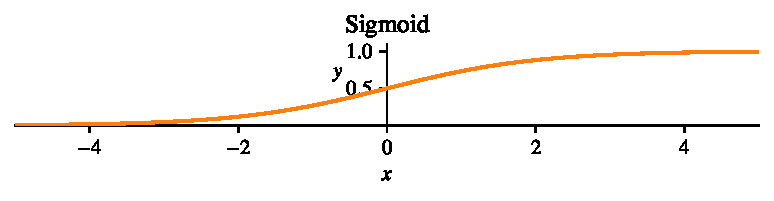
\includegraphics[width=.7\textwidth]{activators/sigmoid.pdf}
    \caption{A plot of the sigmoid and $(0,1)$-clip activation functions on $[-4, 4]$.}
    \label{fig:sigmoid}
\end{figure}

However, the activation functions do not have to be sigmoidal in order to satisfy the requirements for the Universal Approximation Theorem. In fact, it is enough to require that the activation function is non-polynomial \cite{nonpolynomial}. (\small{venter på svar fra Morten, virker for godt til å være sant}) 

Another commonly used activation function is the rectified linear unit (ReLU), defined by
\begin{equation*}
    f(x) = \max(0, x) = \frac{x + |x|}{2} =
    \begin{cases}
        x & \textnormal{if } x \geq 0 \\
        0 & \textnormal{if } x < 0
    \end{cases}.
\end{equation*}
However, this function suffers from what some call dying ReLUs, where nodes in effect die by outputting constant $0$. To combat this, we introduce the leaky rectified linear unit (LReLU), defined by
\begin{equation*}
    f(x) =
    \begin{cases}
        x & \textnormal{if } x \geq 0 \\
        \gamma x & \textnormal{if } x < 0
    \end{cases}.
\end{equation*}
for some positive $\gamma \in \mathbb{R}$. 

\begin{figure}[ht]
    \centering
    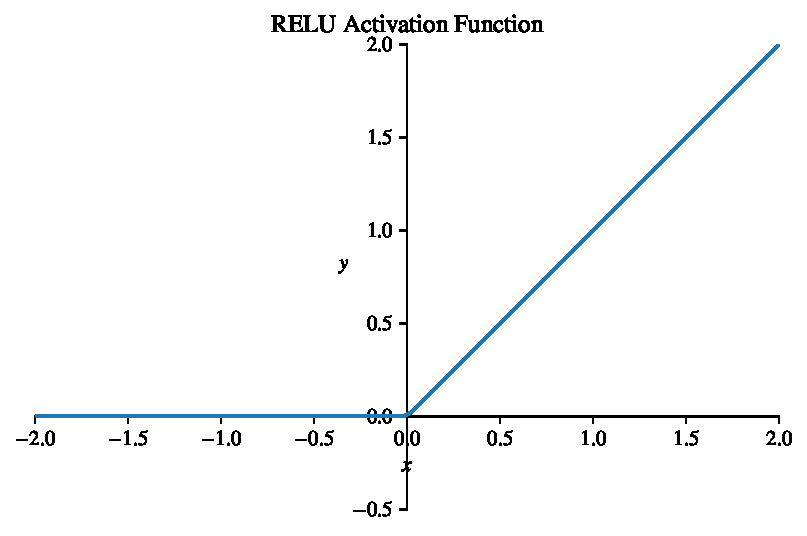
\includegraphics[width=.7\textwidth]{activators/RELU.pdf}
    \caption{A plot of rectified linear unit (ReLU) activation function on $[-2, 2]$.}
    \label{fig:RELU}
\end{figure}

\begin{figure}[ht]
    \centering
    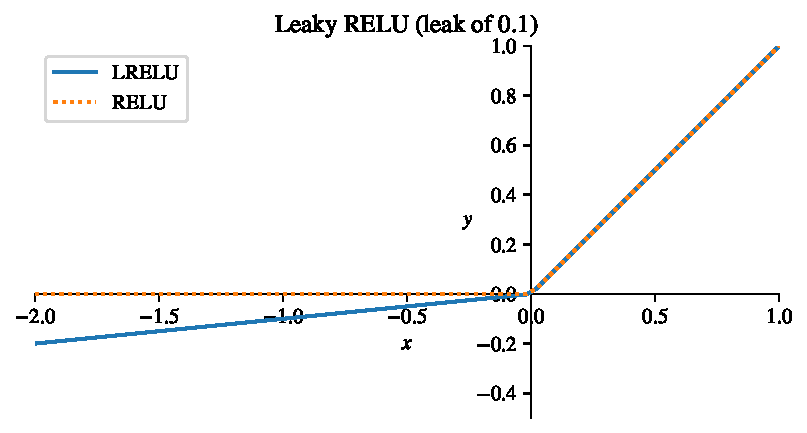
\includegraphics[width=.7\textwidth]{activators/LRELU.pdf}
    \caption{A plot of leaky rectified linear unit (LRELU) activation function on $[-2, 1]$, with $\gamma=0.1$, against RELU.}
    \label{fig:LRELU}
\end{figure}


\subsubsection{Back propagation}

\section{Method}

\section{Results}

\section{Discussion}

\section{Conclusion}

\section{References}

\bibliography{Project2/refs} % add  references to this 

\section{Appendix}
The code is publicly available on \href{https://github.com/augustfe/FYSSTK}{github.com/augustfe/FYSSTK}, written in python.


\end{document}